\documentclass[12pt]{article}
\usepackage[utf8]{inputenc}
\usepackage{geometry}
\geometry{a4paper, top=0.55in, bottom=0.55in, left=0.58in, right=0.58in}
\usepackage{mathptmx}
\usepackage{amsmath, amssymb}
\usepackage{booktabs}
\usepackage{hyperref}
\usepackage{setspace}
\usepackage{graphicx}
\usepackage{float}
\usepackage{multirow}
\usepackage{titlesec}

\setstretch{1.0}

% Tighten section/subsection vertical spacing
\titlespacing*{\section}{0pt}{7pt plus 2pt minus 1pt}{4pt plus 1pt}
\titlespacing*{\subsection}{0pt}{5pt plus 2pt minus 1pt}{3pt plus 1pt}

% Tighten float spacing
\setlength{\floatsep}{4pt}
\setlength{\textfloatsep}{7pt}
\setlength{\intextsep}{4pt}
\setlength{\abovecaptionskip}{3pt}
\setlength{\belowcaptionskip}{0pt}

% Tighten display math spacing
\setlength{\abovedisplayskip}{4pt}
\setlength{\belowdisplayskip}{4pt}
\setlength{\abovedisplayshortskip}{2pt}
\setlength{\belowdisplayshortskip}{2pt}
\title{\vspace{-1.4cm}Cross-Currency Dynamics in Cryptocurrencies \vspace{-0.7cm}}
\date{}

\begin{document}
\maketitle
\vspace{-1.4cm}

\section*{Abstract}
When Silicon Valley Bank collapsed in March 2023, USDC briefly traded at \$0.87, fragmenting Bitcoin prices across exchanges and quote currencies. Using 1-minute data from Binance, Coinbase, and Kraken, we show that this fragmentation splits cleanly into a large stablecoin-driven component---raw cross-currency gaps reaching $+320$ basis points---and a small residual of just $+5$ bps once the stablecoin leg is marked to USD, which mean-reverts in under one minute. Simultaneously, USDT traded at a premium as traders rotated away from USDC, and volume migrated toward USD and USDT pairs, confirming a system-wide flight-to-quality response. Fiat-quoted BTC leads price discovery over USDT-quoted BTC on Kraken, while the USDC channel does not establish a stable cointegrating relationship over our window. Fee-only crisis arbitrage profitability of 29\% in the USDC channel shrinks to 7\% under realistic slippage, confirming genuine cross-venue opportunities are narrow even at peak stress. These findings show that stablecoin reserve credibility---the target of the 2025 GENIUS Act---is the key lever for reducing the banking-layer fragility that drives cross-venue pricing fragmentation.

\section{Context and Motivation}

Stablecoins are the primary quote currency on most crypto exchanges, functioning as digital cash accounts that traders use to quote prices, move liquidity, and fund positions across venues. Because stablecoins are not identical to bank deposits---redeemability, custody, and transparency can differ---their prices can deviate from \$1 and introduce a \emph{stablecoin funding risk premium}: the same underlying asset (BTC) then trades at different nominal prices across quote currencies (BTC/USD vs.\ BTC/USDC vs.\ BTC/USDT) purely because of stablecoin-specific risk. In 2025, the U.S.\ enacted the GENIUS Act, establishing a federal framework for dollar-pegged stablecoins with stricter reserve backing and transparency, targeting exactly this channel.

To study how stablecoin stress affects pricing, we analyze March 1--21, 2023 (UTC), which includes the SVB failure. When SVB collapsed on March 10, approximately \$3.3B of Circle's USDC reserves became temporarily inaccessible, and USDC de-pegged to as low as \$0.87 on March 11--12. This episode provides a clean, high-frequency stress test of cross-currency basis behavior, liquidity fragmentation, and price discovery---and a natural case study for what the GENIUS Act is designed to prevent.

\section{Data and Methodology}

\subsection{Data sources and preprocessing}
We collect 1-minute OHLCV candles for BTC quoted in USD, USDT, and USDC from three centralized exchanges chosen for their distinct regulatory exposure and market structure. Binance provides BTC/USDT and BTC/USDC and dominates global USDT volume. Coinbase provides BTC/USD, BTC/USDT, and USDT/USD and serves as a primary U.S.\ fiat gateway. Kraken provides BTC/USD, BTC/USDT, BTC/USDC, USDT/USD, and USDC/USD, offering the broadest set of stablecoin-to-fiat legs. BTC/EUR pairs are collected for completeness but are not central to the results. For stablecoin-to-USD conversion in $B_t$, we use venue-specific legs (e.g., Kraken USDC/USD for Kraken channels). All series are aligned to a unified 1-minute UTC grid; coverage ranges from about 94\% to above 99\%, with most series above 98\%. Short micro-gaps (up to 5 minutes) are forward-filled; larger gaps are flagged.

We proxy transaction frictions using the intra-candle range:
\begin{equation}
    \text{Intra-minute Range (bps)} = \left( \frac{\text{High}_t - \text{Low}_t}{\text{Close}_t} \right)\times 10000.
\end{equation}
This is a coarse range proxy that mechanically loads on volatility and microstructure noise; we interpret it cautiously as a friction indicator, not a quoted bid--ask spread.

\subsection{Core quantitative objects}

For stablecoin $Q\in\{\text{USDC}, \text{USDT}\}$, we track two objects. The \emph{unadjusted dispersion}:
\begin{equation}
    D_{Q,t}=\left(\ln(P_{\text{BTC}/Q,t})-\ln(P_{\text{BTC/USD},t})\right)\times 10000,
\end{equation}
and the \emph{adjusted parity residual}:
\begin{equation}
    B_{Q,t}
    = \left(\ln(P_{\text{BTC}/Q,t}\times P_{Q/\text{USD},t})-\ln(P_{\text{BTC/USD},t})\right)\times 10000.
\end{equation}
These satisfy $B_{Q,t}=D_{Q,t}+10000\cdot\ln(P_{Q/\text{USD},t})$, so large stablecoin de-pegs mechanically drive $D_t$ while $B_t$ captures the residual after marking the stablecoin leg to USD. Both objects are computed intra-exchange to isolate stablecoin effects from venue differences; cross-venue deviations are studied separately as cross-exchange log-price differentials.

\subsection{Mean reversion via Ornstein--Uhlenbeck}
We model $B_t$ as an OU process $dX_t = \theta(\mu - X_t)dt + \sigma dW_t$ and estimate the discrete AR(1) form $X_t = c + \rho X_{t-1} + \varepsilon_t$. Stationarity is checked with ADF tests (with large $N$, rejection is expected and serves as a baseline screen). The half-life uses the exact mapping:
\begin{equation}
    \tau_{1/2} = \frac{\ln(2)\,\Delta t}{-\ln(\rho)}, \quad 0<\rho<1.
\end{equation}
If $\rho \le 0$ or $\rho \ge 1$, half-life is undefined (NaN). We report robustness at 5-minute sampling and with forward-filled minutes removed.

\subsection{Price discovery: Johansen + VECM (primary) and Granger (secondary)}
For the two primary Kraken channels (BTC/USD vs.\ BTC/USDC and BTC/USD vs.\ BTC/USDT), we use synchronized 1-minute log-price levels, dropping forward-filled minutes. We test for cointegration with Johansen trace tests (constant restricted to the cointegration relation; lag order via BIC on the levels VAR). When rank $=1$, we estimate:
\begin{equation}
    \Delta \mathbf{p}_t = \alpha \beta^\top \mathbf{p}_{t-1} + \sum_{i=1}^{k_{\Delta}} \Gamma_i \Delta \mathbf{p}_{t-i} + \mathbf{u}_t.
\end{equation}
The market with smaller $|\alpha|$ adjusts less and is interpreted as the relative leader. We retain BH/FDR-corrected Granger tests on returns as secondary evidence only; with 1-minute bars, asynchrony and large $N$ can overstate economic lead--lag strength.

\section{Empirical Results}

\subsection{Dispersion, adjusted residual, and mean reversion}

Before SVB (March 1--9), both $D_t$ and $B_t$ are near zero on Kraken. During the crisis (March 10--13), the \emph{unadjusted} USDC dispersion jumps to mean $+319.97$ bps ($\sigma=322.87$), while the \emph{adjusted} USDC residual is much smaller (mean $+5.27$ bps, $\sigma=21.21$). USDT shows smaller dislocations in the opposite direction: crisis $D_t=-57.18$ bps, $B_t=+0.68$ bps (Table~\ref{tab:dispersion_vs_adjusted}). This asymmetry reflects two simultaneous dynamics: USDC trades as low as \$0.87 on March 11 (${\approx}{-}1{,}300$ bps), mechanically inflating $D_t$, while USDT simultaneously trades at a \emph{premium} to \$1---averaging $+58.1$ bps on Kraken and $+59.7$ bps on Coinbase during March 10--13. The USDT premium is consistent with a flight-to-quality rotation within the stablecoin market: as USDC lost its peg, traders moved into USDT as the more trusted alternative, pushing its price above \$1. The two stablecoins thus acted as imperfect substitutes under stress, with demand rotating from one to the other rather than evaporating.

\begin{figure}[H]
    \centering
    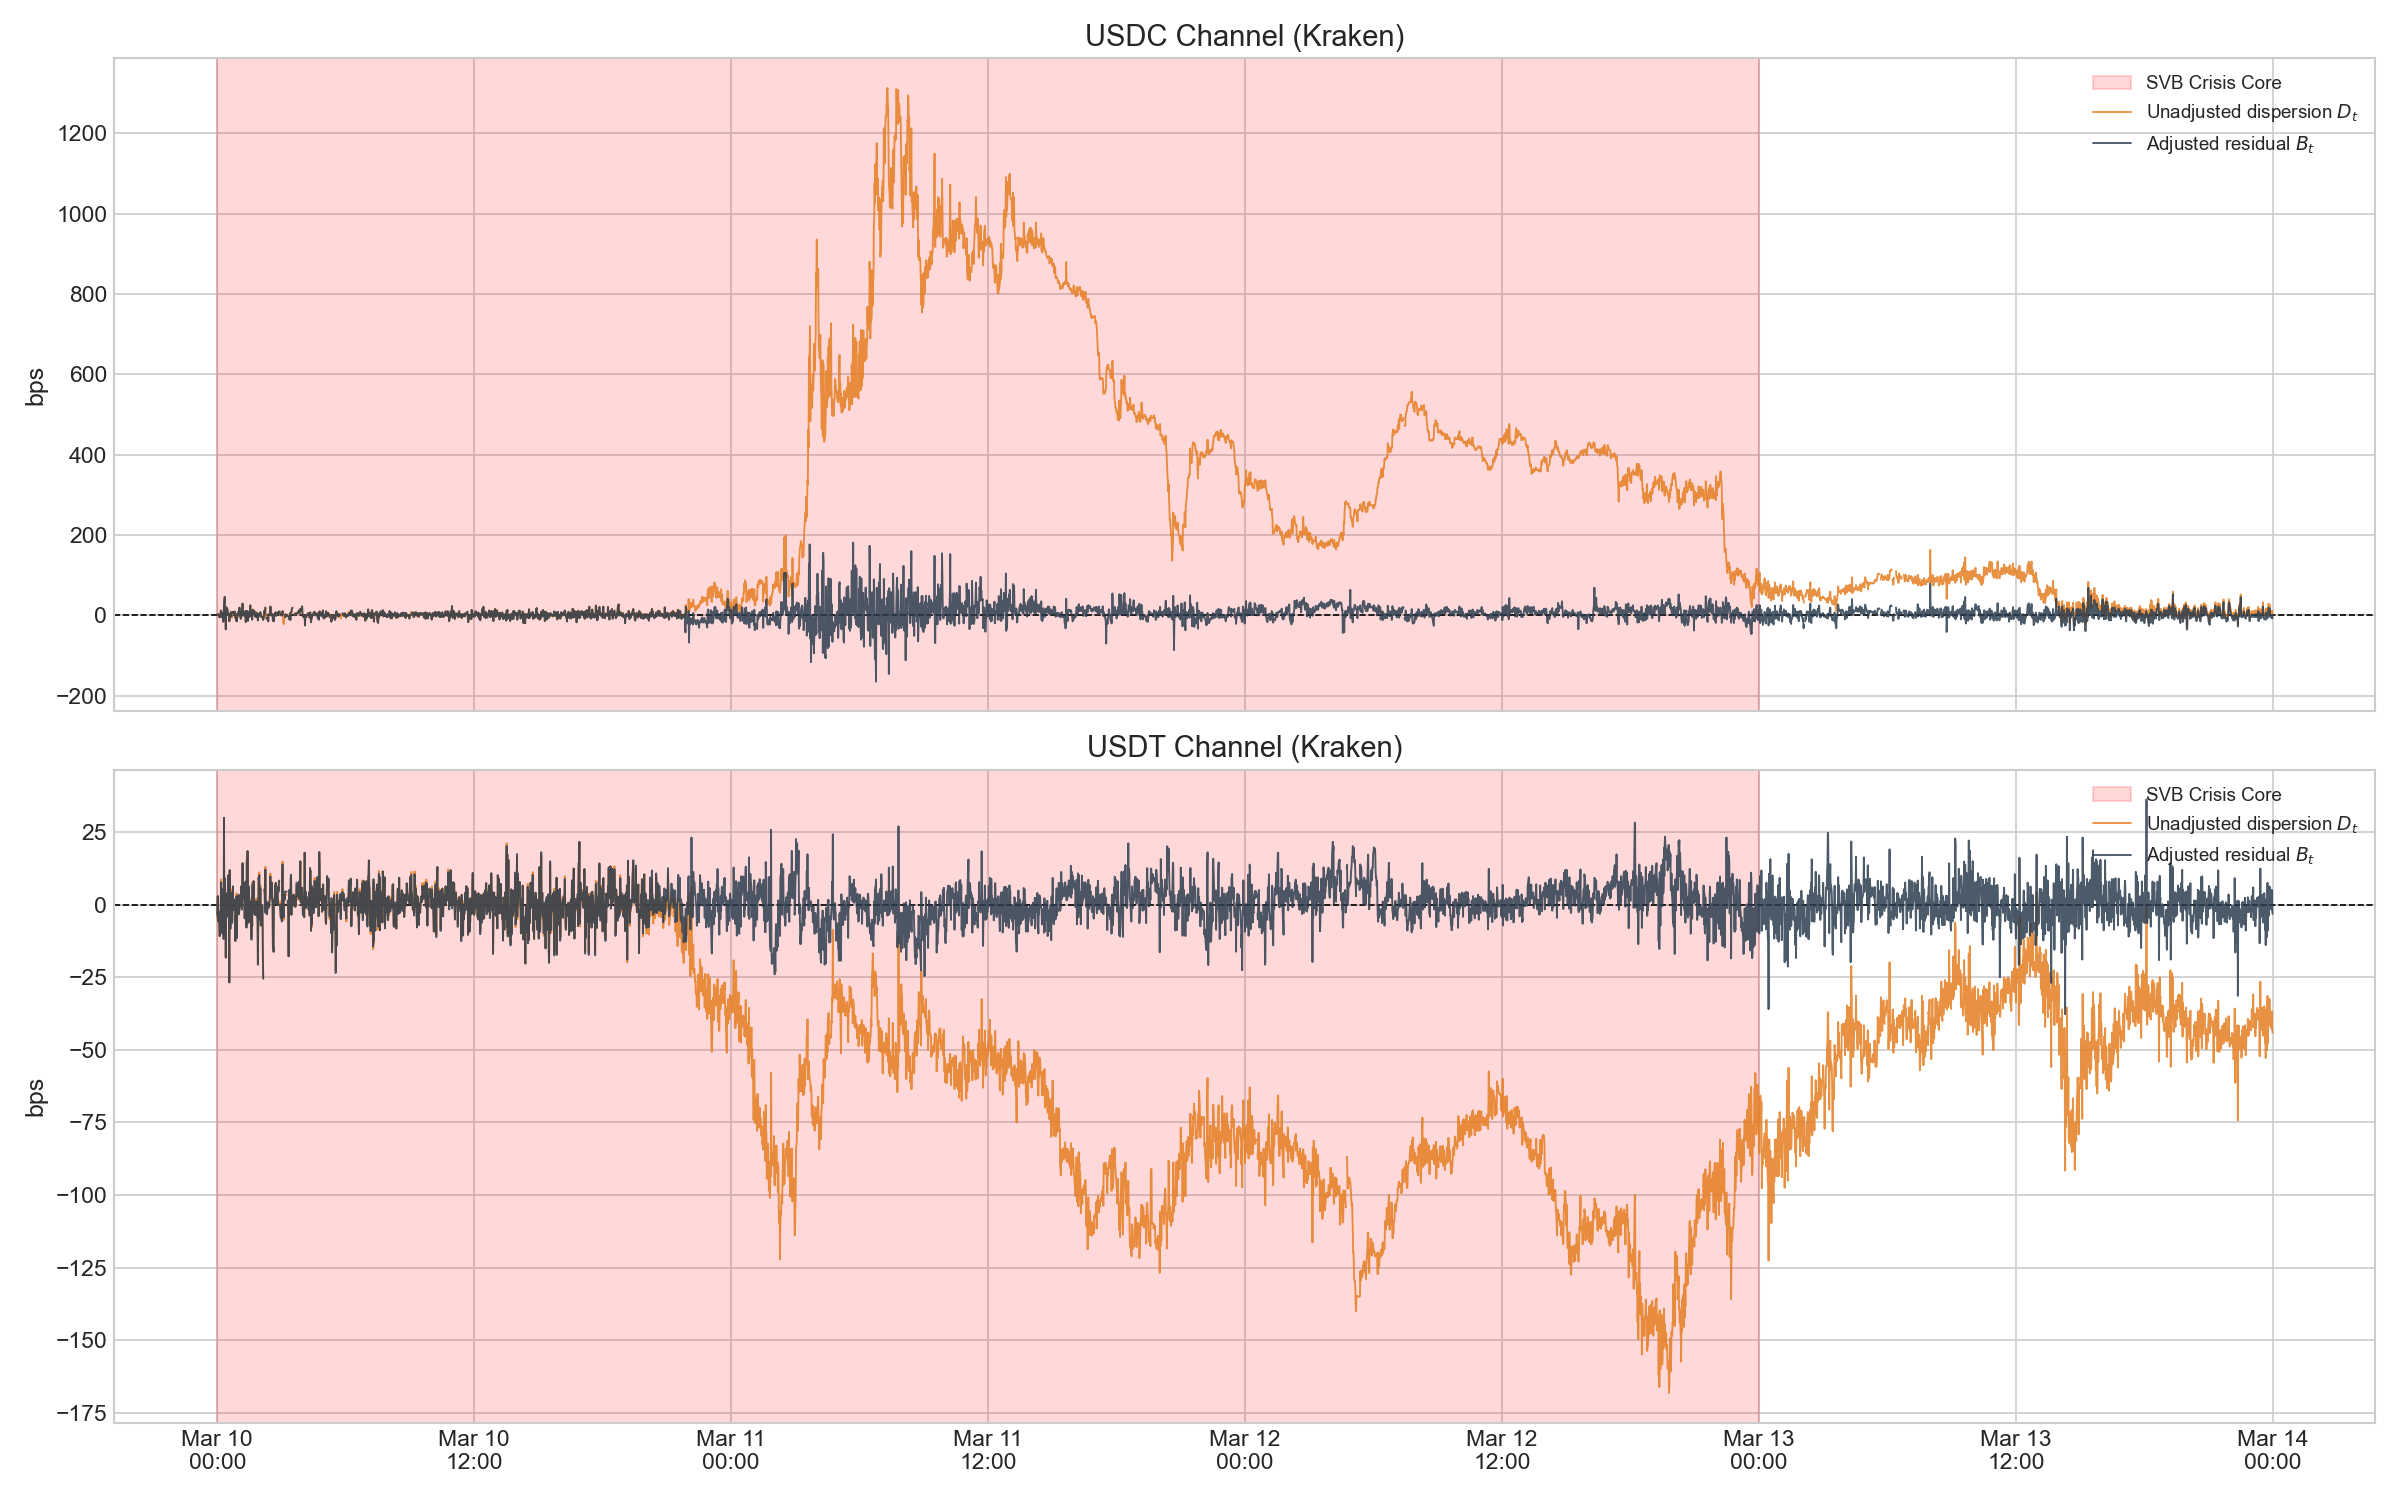
\includegraphics[width=0.75\linewidth]{figures/fig_dispersion_vs_adjusted_kraken.png}
    \caption{SVB window (March 10--13): unadjusted dispersion $D_t$ vs.\ adjusted residual $B_t$ on Kraken. The USDC de-peg dominates $D_t$, while $B_t$ remains far smaller after marking the stablecoin leg to USD.}
    \label{fig:disp_vs_adj}
\end{figure}

\input{tables/dispersion_adjusted_stats.tex}

ADF rejects a unit root for all $B_t$ channels ($p<0.001$). Using the exact half-life mapping, the USDC adjusted residual on Kraken has half-life $0.98$ min pre-SVB, $0.61$ min in crisis, and $0.79$ min post-SVB (1-minute, all observations). Robustness across sampling frequencies (1m, 5m) and forward-fill filters confirms USDC crisis half-life ranges from $0.54$ to $1.10$ minutes; USDT crisis half-life is longer ($0.92$--$3.06$ min). Fast USDC mean reversion is robust, though whether crisis half-life strictly falls relative to calm is specification-sensitive.

\begin{figure}[H]
    \centering
    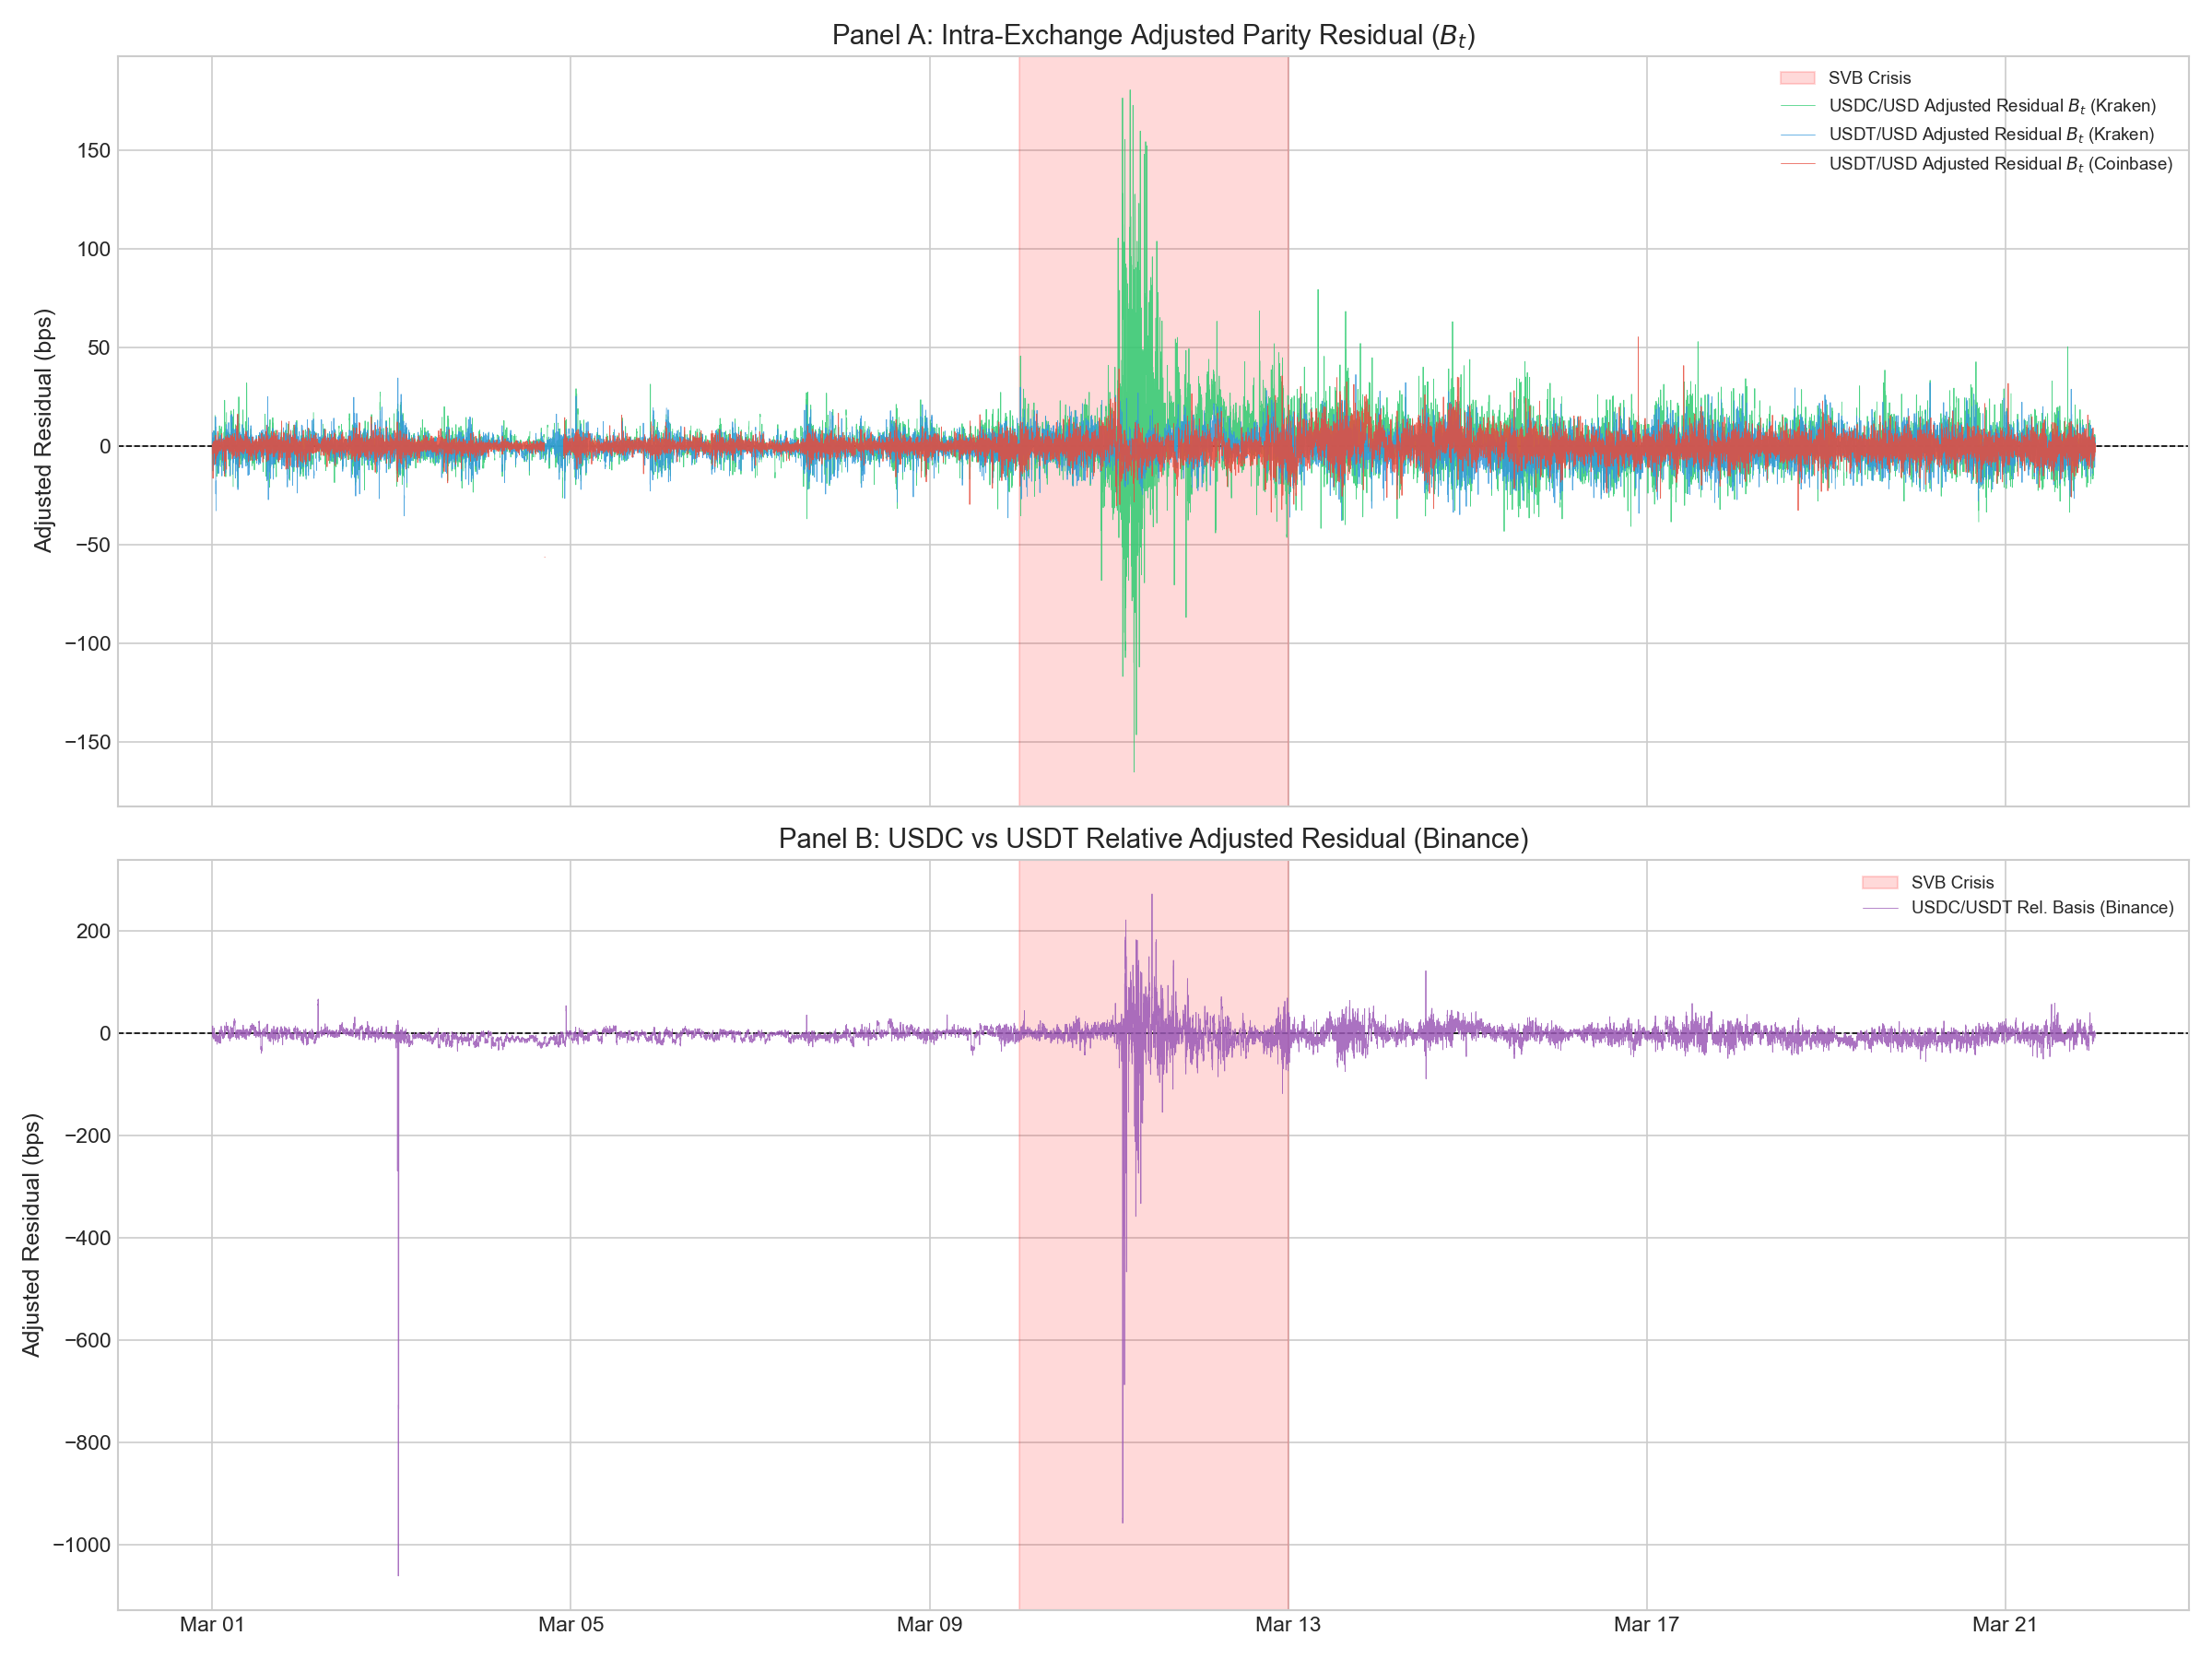
\includegraphics[width=0.69\linewidth]{figures/fig_basis_timeseries.png}
    \caption{Panel A: intra-exchange adjusted parity residuals ($B_t$) on Kraken and Coinbase. Panel B: USDC/USDT relative adjusted residual on Binance.}
    \label{fig:basis_ts}
\end{figure}

\begin{figure}[H]
    \centering
    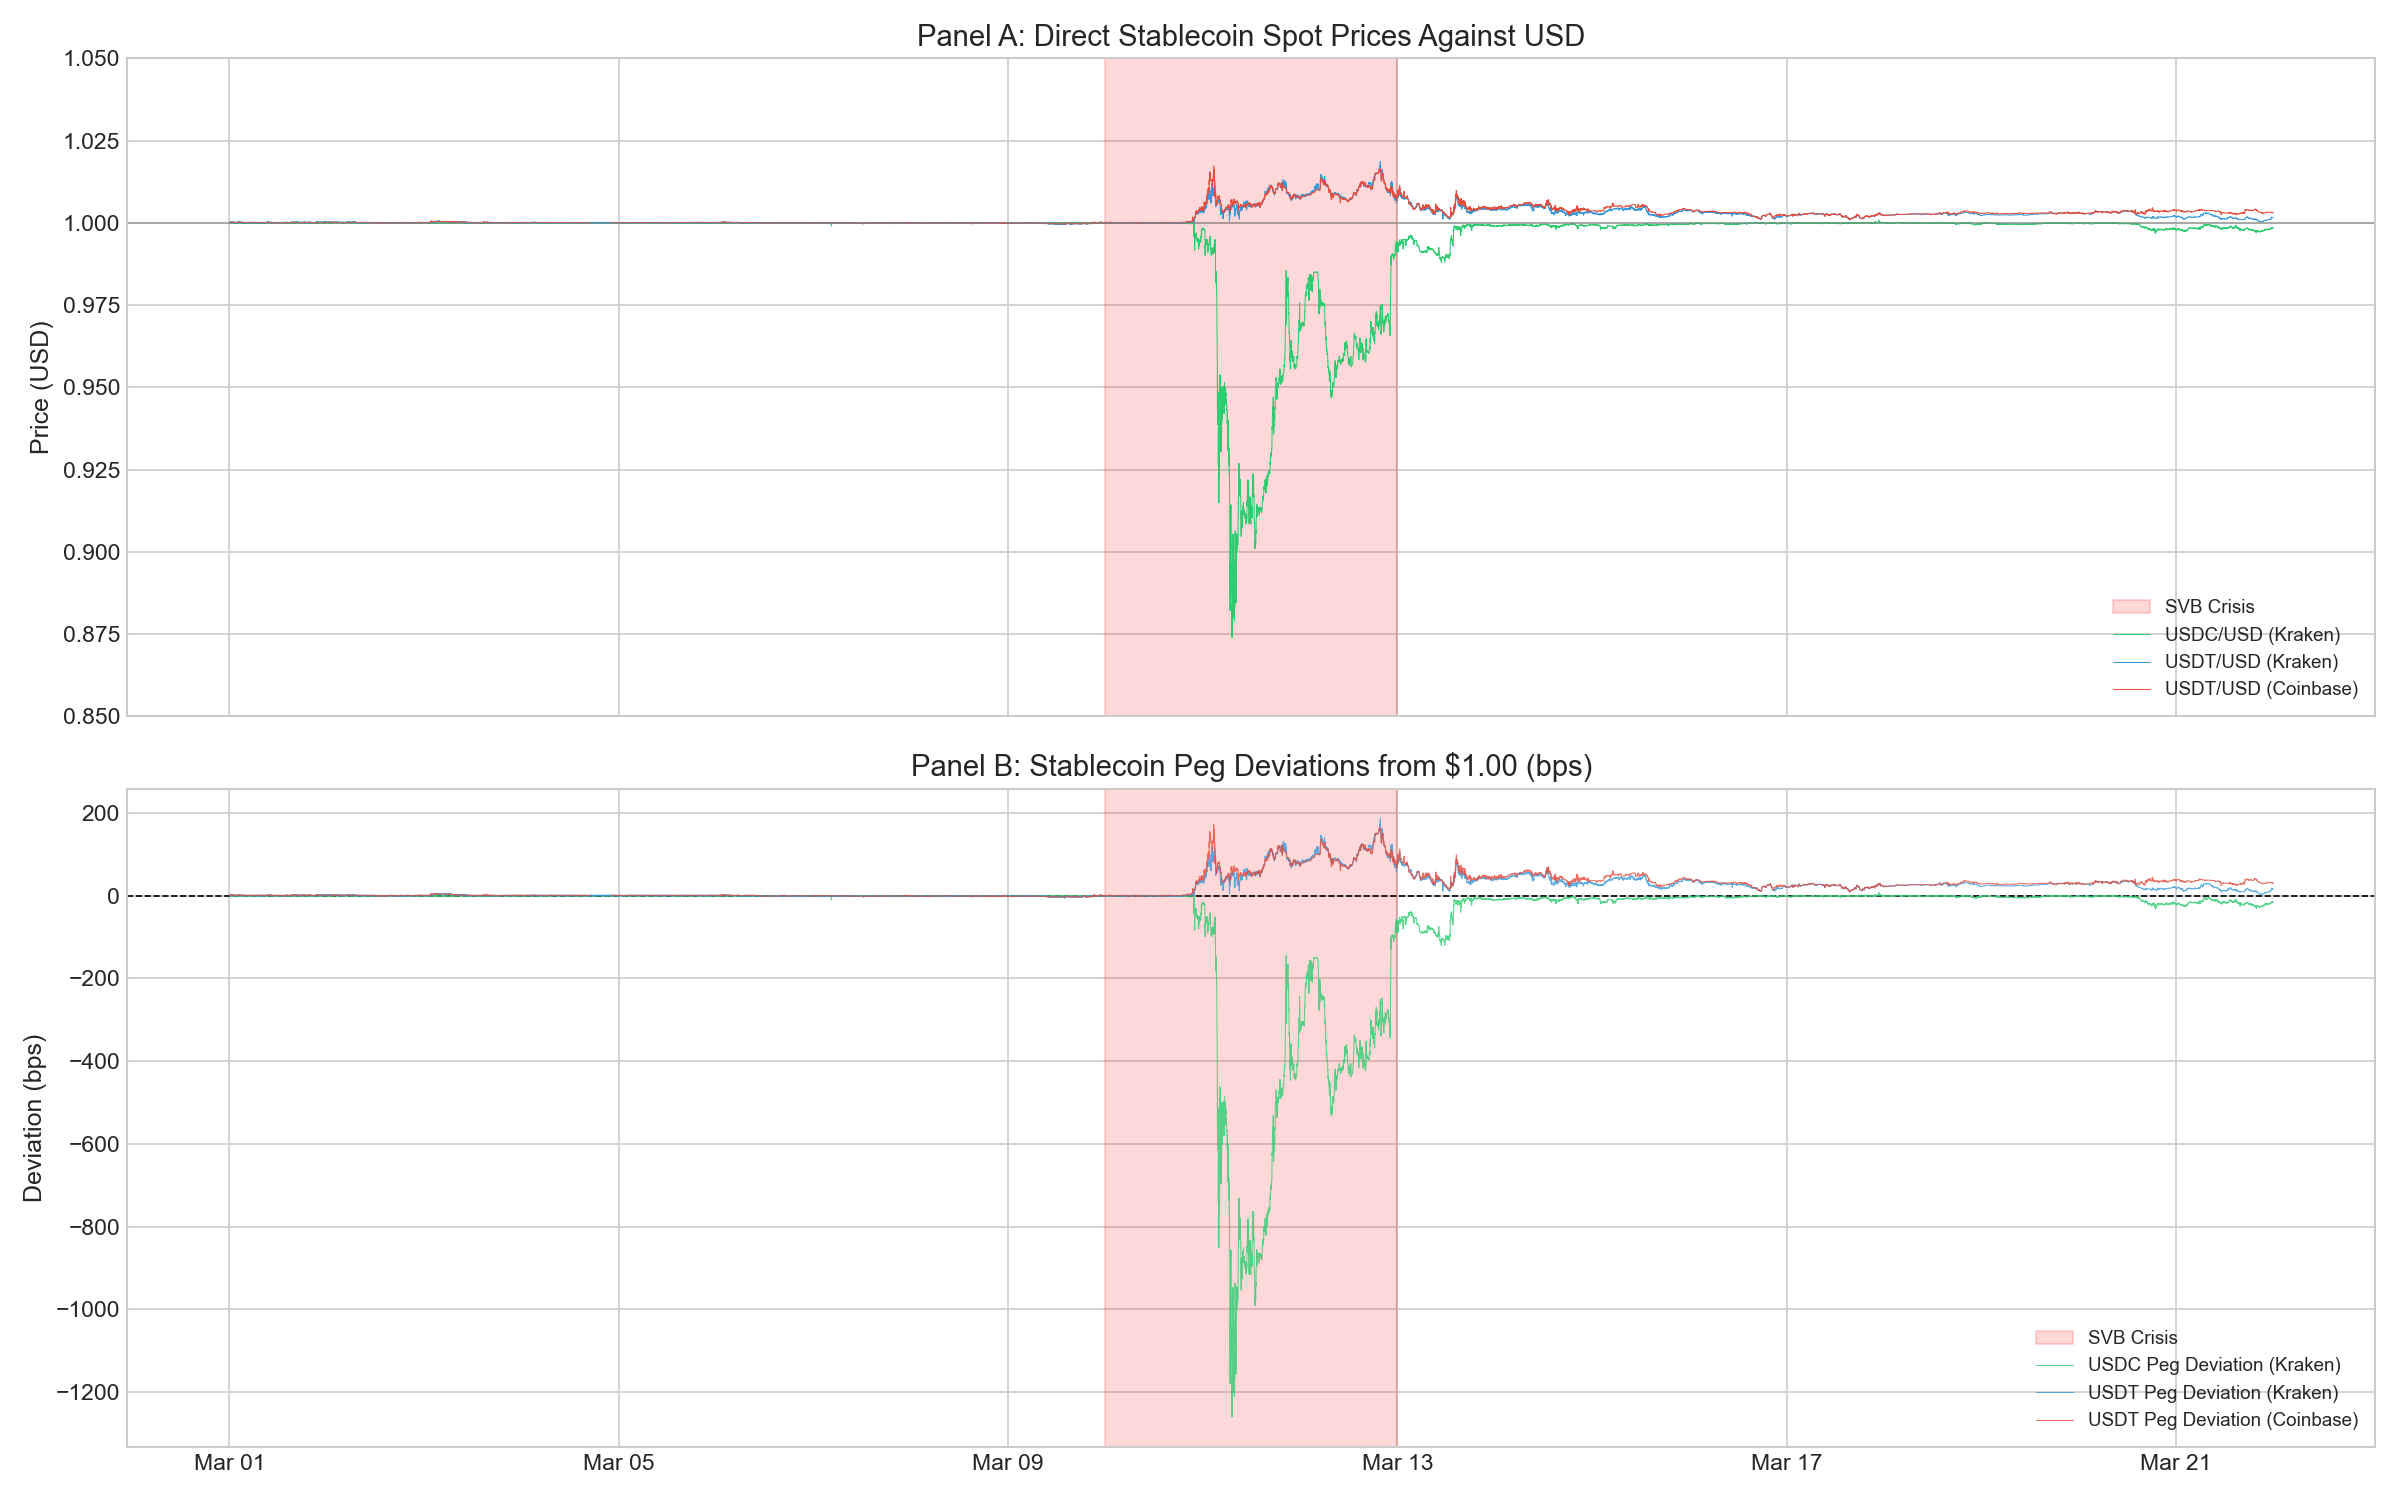
\includegraphics[width=0.85\linewidth]{figures/fig_stablecoin_peg.png}
    \caption{Panel A: stablecoin spot prices vs.\ USD. Panel B: peg deviations from \$1.00 (bps). USDC falls sharply while USDT trades at a premium, consistent with a flight-to-quality rotation within the stablecoin market.}
    \label{fig:peg}
\end{figure}

\subsection{Cross-exchange spatial arbitrage}
We compute log-price differentials for BTC/USDT (Binance vs.\ Kraken; Coinbase vs.\ Kraken) and BTC/USD (Coinbase vs.\ Kraken). An important caveat applies to the USDT cross-exchange channel: it captures dispersion in the USDT numeraire, so a USD-based arbitrage would require an additional USDT/USD conversion leg unless USDT/USD quotes are identical across venues. In calm periods, Binance--Kraken BTC/USDT deviations are near zero (mean $0.007$ bps), confirming efficient cross-venue arbitrage in this liquid channel; Coinbase--Kraken BTC/USD shows a persistent positive mean ($+2.18$ bps), consistent with a structural premium on the primary U.S.\ fiat gateway.

\begin{figure}[H]
    \centering
    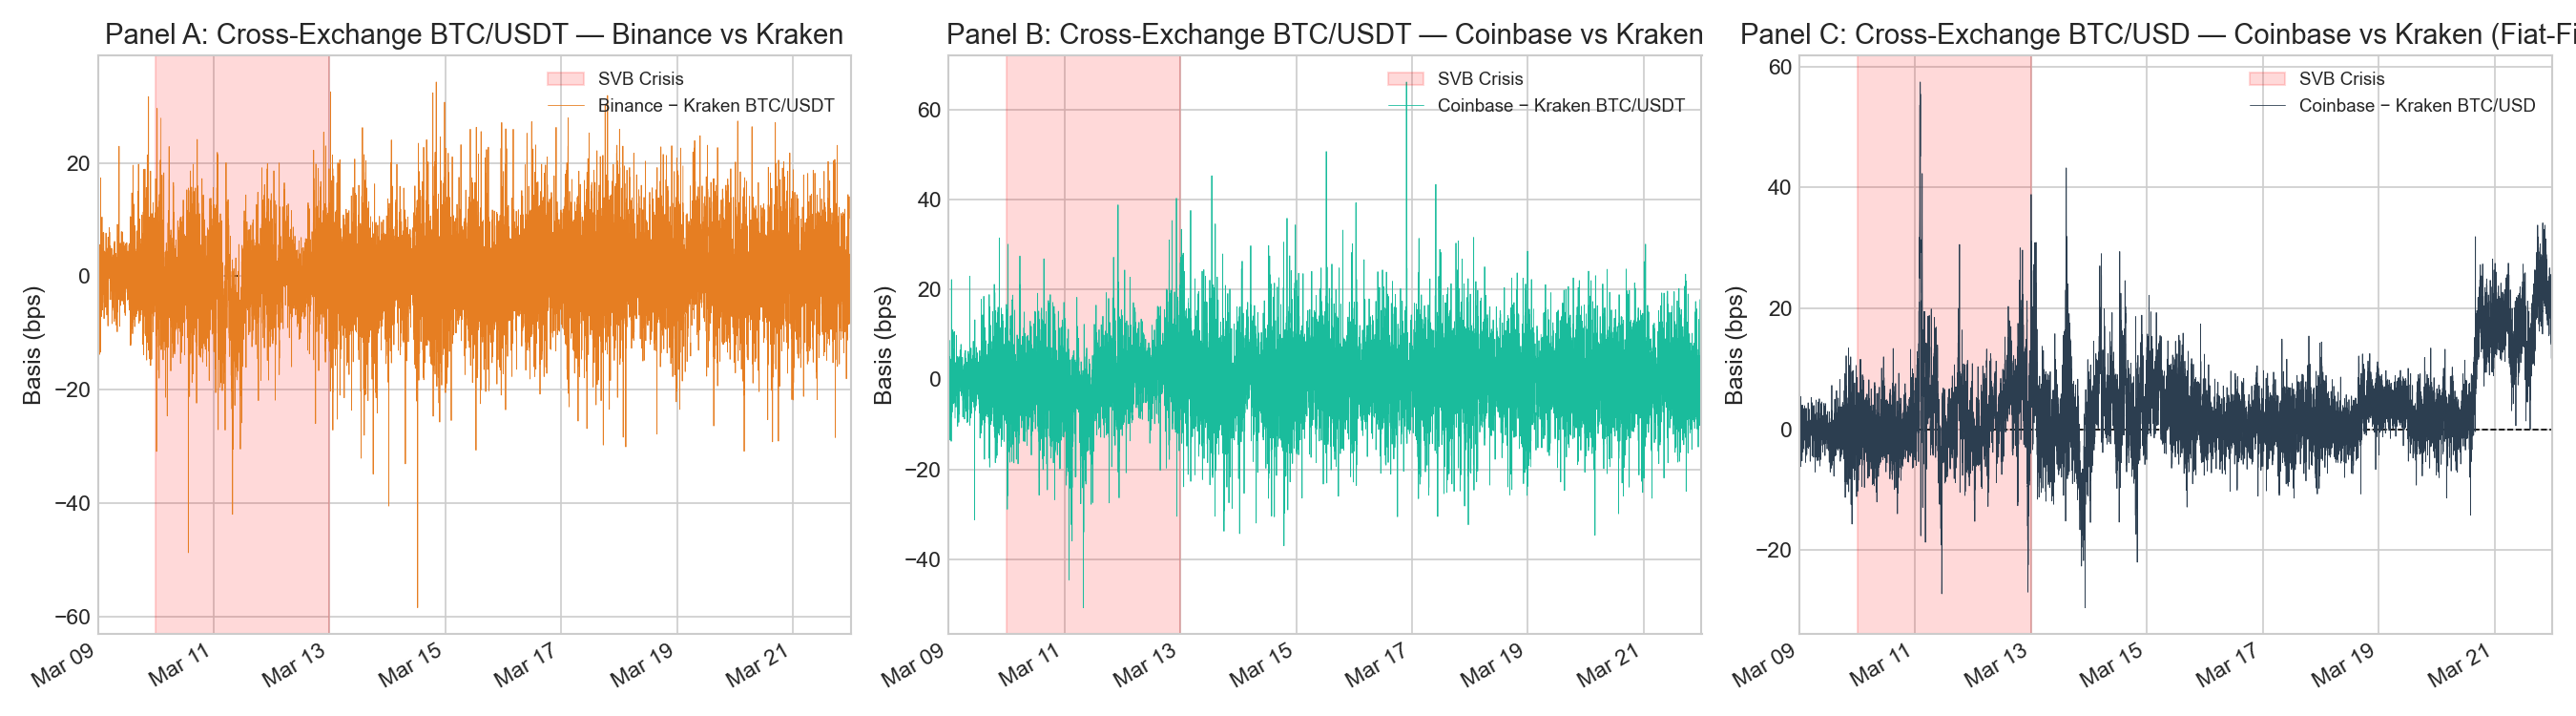
\includegraphics[width=0.84\linewidth]{figures/fig_cross_exchange_basis.png}
    \caption{Cross-exchange basis: BTC/USDT (Binance vs.\ Kraken, Coinbase vs.\ Kraken) and BTC/USD (Coinbase vs.\ Kraken). The fiat channel (Panel C) shows a persistent positive basis that remains elevated post-crisis.}
    \label{fig:xbasis}
\end{figure}

During the crisis, all cross-exchange differentials widen simultaneously alongside the intra-exchange $B_t$ deviations (visible in Figures~\ref{fig:basis_ts} and~\ref{fig:xbasis}). The co-movement of intra- and cross-exchange dislocations indicates system-wide stress rather than a single-venue disruption. Notably, the Coinbase--Kraken fiat premium did not fully normalize after the crisis, suggesting it partly reflects structural microstructure differences that stress amplified rather than created.

\subsection{Liquidity, volatility, and volume dynamics}
We quantify liquidity across quote currencies using two standard microstructure estimators applied to the same 1-minute data. The Roll (1984) effective spread uses the daily serial covariance of log returns: $\hat{s}_t = 2\sqrt{-\text{Cov}(\Delta p_t,\Delta p_{t-1})}$, expressed in basis points. The Amihud (2002) illiquidity ratio $\text{ILLIQ}_t = |r_t|/\text{DollarVol}_t$ measures price impact per dollar traded. Together they capture two distinct liquidity dimensions: microstructure frictions (Roll) and market depth (Amihud).

Table~\ref{tab:liquidity_spread} and Figure~\ref{fig:liq} report regime-level means. The Roll spread for Kraken BTC/USDC jumps from $1.10$ bps pre-crisis to $25.64$ bps during the SVB window---a $23\times$ increase---while Kraken BTC/USDT holds near $3$ bps throughout. The Roll estimator requires negative serial covariance (bid-ask bounce); for Kraken BTC/USD during the crisis the covariance turns non-negative, consistent with sustained price-momentum as BTC recovered from the March 10 selloff. The Amihud ILLIQ confirms that Coinbase BTC/USD is the deepest market across all regimes ($\text{ILLIQ}<0.01$), while Kraken BTC/USDC carries the highest price-impact cost even in calm periods ($\text{ILLIQ}=31.97$ pre-crisis), suggesting structurally thinner liquidity in the USDC channel that amplified when the peg broke.

\begin{figure}[H]
    \centering
    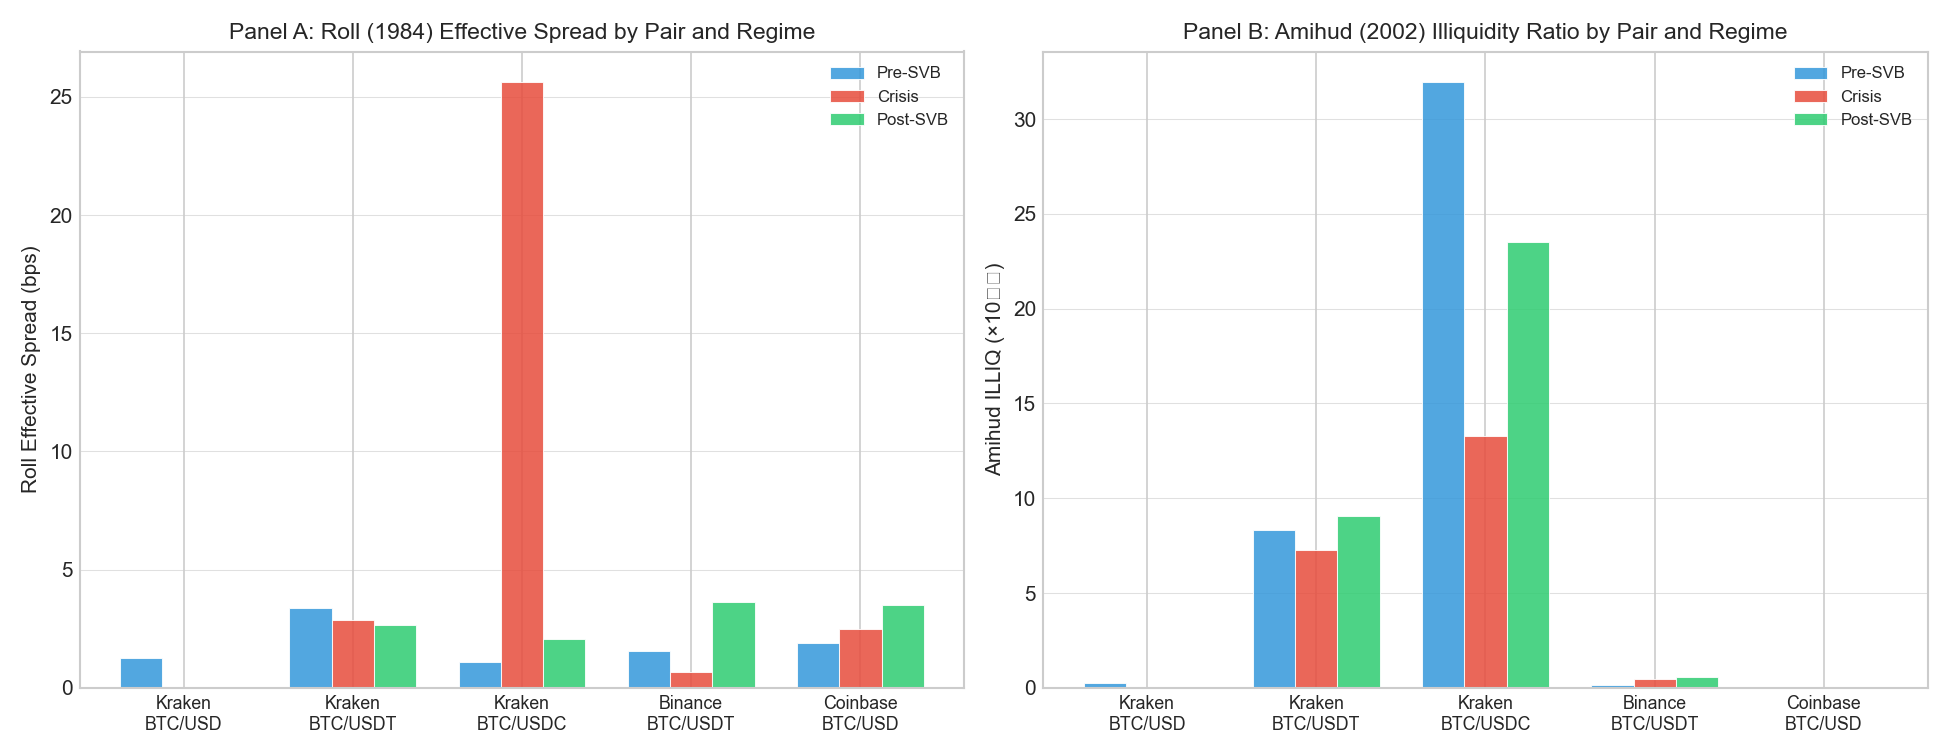
\includegraphics[width=0.78\linewidth]{figures/fig_liquidity_roll_amihud.png}
    \caption{Panel A: Roll (1984) effective spread by pair and regime (bps). Panel B: Amihud (2002) ILLIQ ratio ($\times 10^{-6}$). Kraken BTC/USDC shows a $23\times$ Roll spread increase during the crisis; Roll is undefined for Kraken BTC/USD in stress periods (positive serial covariance, momentum regime).}
    \label{fig:liq}
\end{figure}

\input{tables/liquidity_spread_table.tex}

HAC regressions (Newey--West, 60 lags) of $B_t$ on a crisis dummy, realized volatility, and intra-minute range (Table~\ref{tab:regression_hac}) confirm the crisis dummy is large and significant for USDC ($+4.30$ bps, $p<0.001$), consistent with the Roll spread and Amihud evidence.

\begin{table}[H]
\caption{HAC Regressions of Adjusted Residual $B_t$ on Crisis Dummy, Realized Volatility, and Range Proxy (Kraken, Newey--West 60 lags)}
\label{tab:regression_hac}
\footnotesize
\centering
\begin{tabular}{lcccc}
\toprule
 & \multicolumn{2}{c}{USDC Channel} & \multicolumn{2}{c}{USDT Channel} \\
\cmidrule(lr){2-3} \cmidrule(lr){4-5}
 & Coef. & $p$-value & Coef. & $p$-value \\
\midrule
Constant          & $+0.166$ & 0.787 & $-0.847$ & $<0.001$ \\
Crisis            & $+4.372$ & $<0.001$ & $+1.668$ & $<0.001$ \\
RealizedVol (60m) & $-0.004$ & 0.942 & $-0.022$ & 0.335 \\
Range Proxy       & $+0.050$ & 0.006 & $-0.011$ & 0.130 \\
\midrule
$R^2$             & \multicolumn{2}{c}{0.042} & \multicolumn{2}{c}{0.012} \\
$N$               & \multicolumn{2}{c}{14,895} & \multicolumn{2}{c}{22,901} \\
\bottomrule
\multicolumn{5}{l}{\footnotesize OLS with HAC standard errors (Newey--West, 60 lags). Dependent variable: $B_t$ (bps).}
\end{tabular}
\end{table}


Volume dynamics tell a complementary story (Figure~\ref{fig:vol_share}). During the crisis, daily volume shifted away from USDC-quoted pairs toward USD and USDT pairs as traders reduced exposure to the de-pegged stablecoin. This reallocation reinforces the flight-to-quality interpretation: participants actively redirected their trading activity, not just prices, in response to USDC reserve uncertainty---and the USDT premium documented above is part of the same dynamic.

\begin{figure}[H]
    \centering
    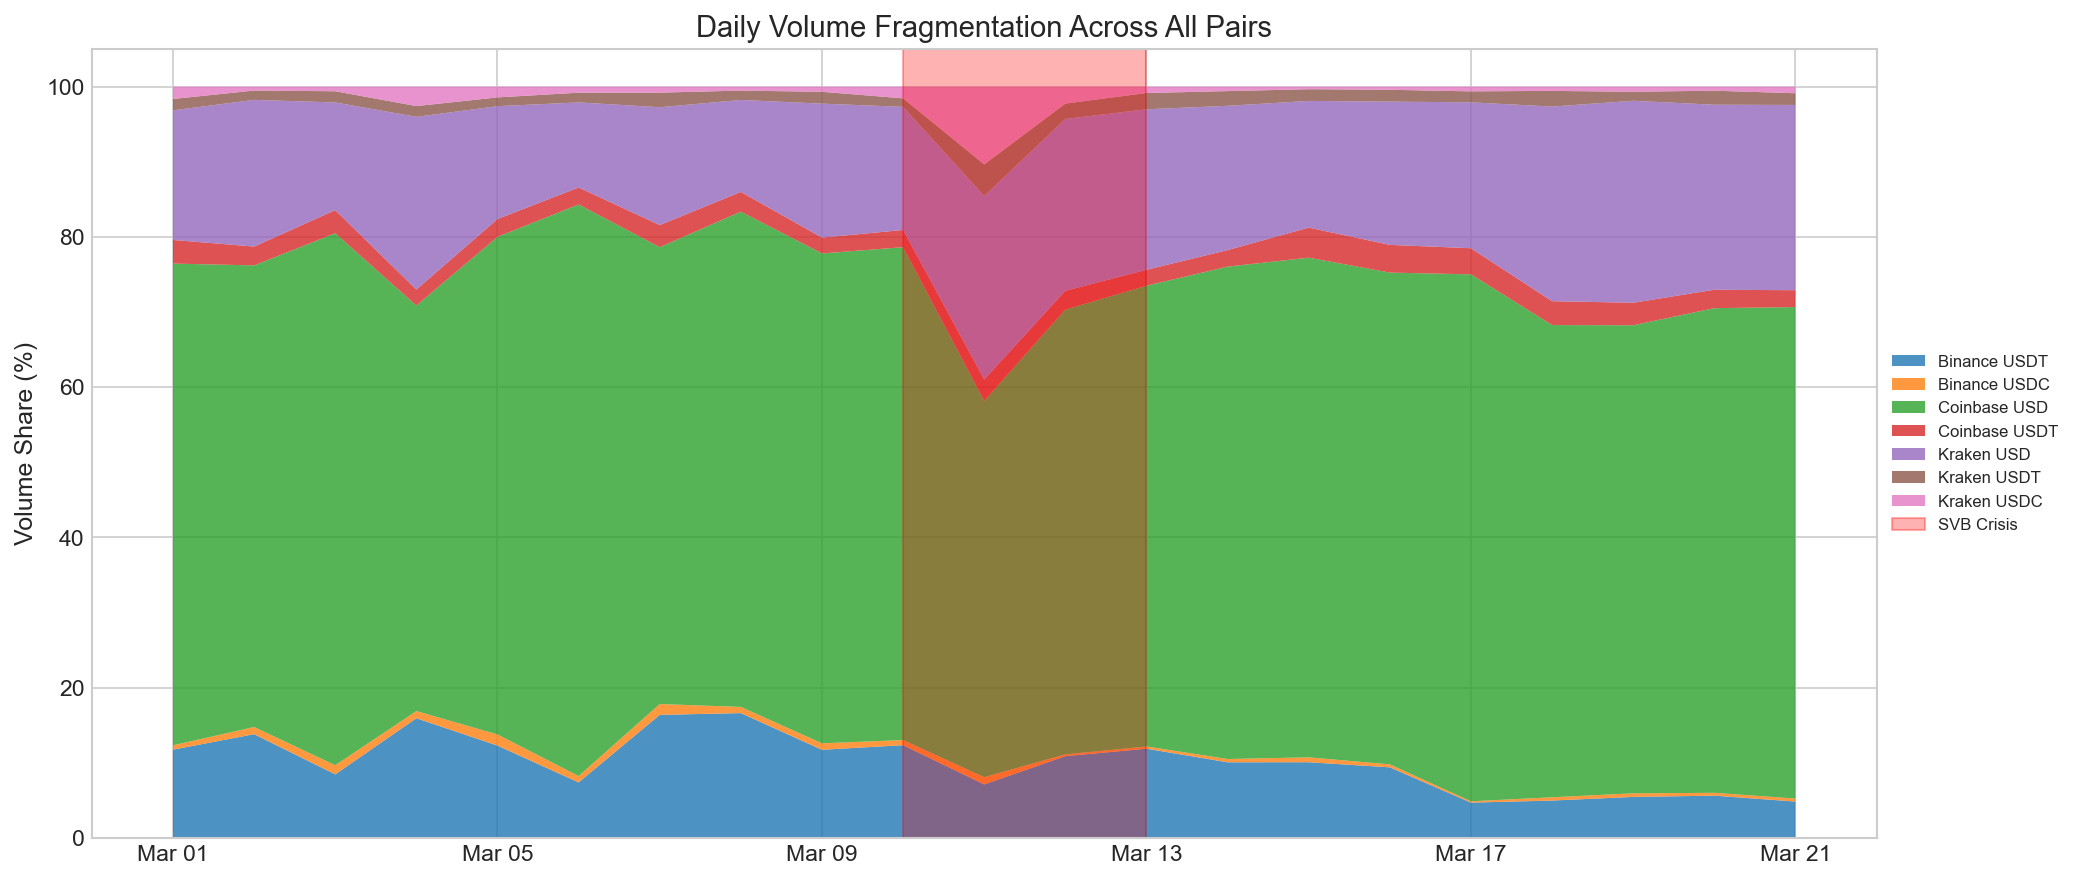
\includegraphics[width=0.82\linewidth]{figures/fig_volume_share.png}
    \caption{Daily volume shares across exchange--pair combinations. Trading shifted toward USD and USDT pairs and away from USDC during the SVB crisis window.}
    \label{fig:vol_share}
\end{figure}

Realized volatility (60-minute rolling standard deviation of 1-minute log returns, scaled to bps/hr via $\sqrt{60}$) reveals pronounced asymmetry across quote currencies (Figure~\ref{fig:rvol}). Kraken BTC/USDC peaks at ${\approx}650$ bps/hr on March 11---roughly $4\times$ the contemporaneous volatility of BTC/USD and BTC/USDT pairs---while non-USDC pairs co-move tightly throughout the window. This excess volatility reflects the compounding of asset risk and numeraire risk: traders in BTC/USDC face BTC price moves and stablecoin peg uncertainty simultaneously, and the two sources of variation are positively correlated during the crisis (both driven by the reserve-confidence shock). Post-crisis, USDC volatility normalizes but remains slightly elevated, consistent with slow full peg recovery.

\begin{figure}[H]
    \centering
    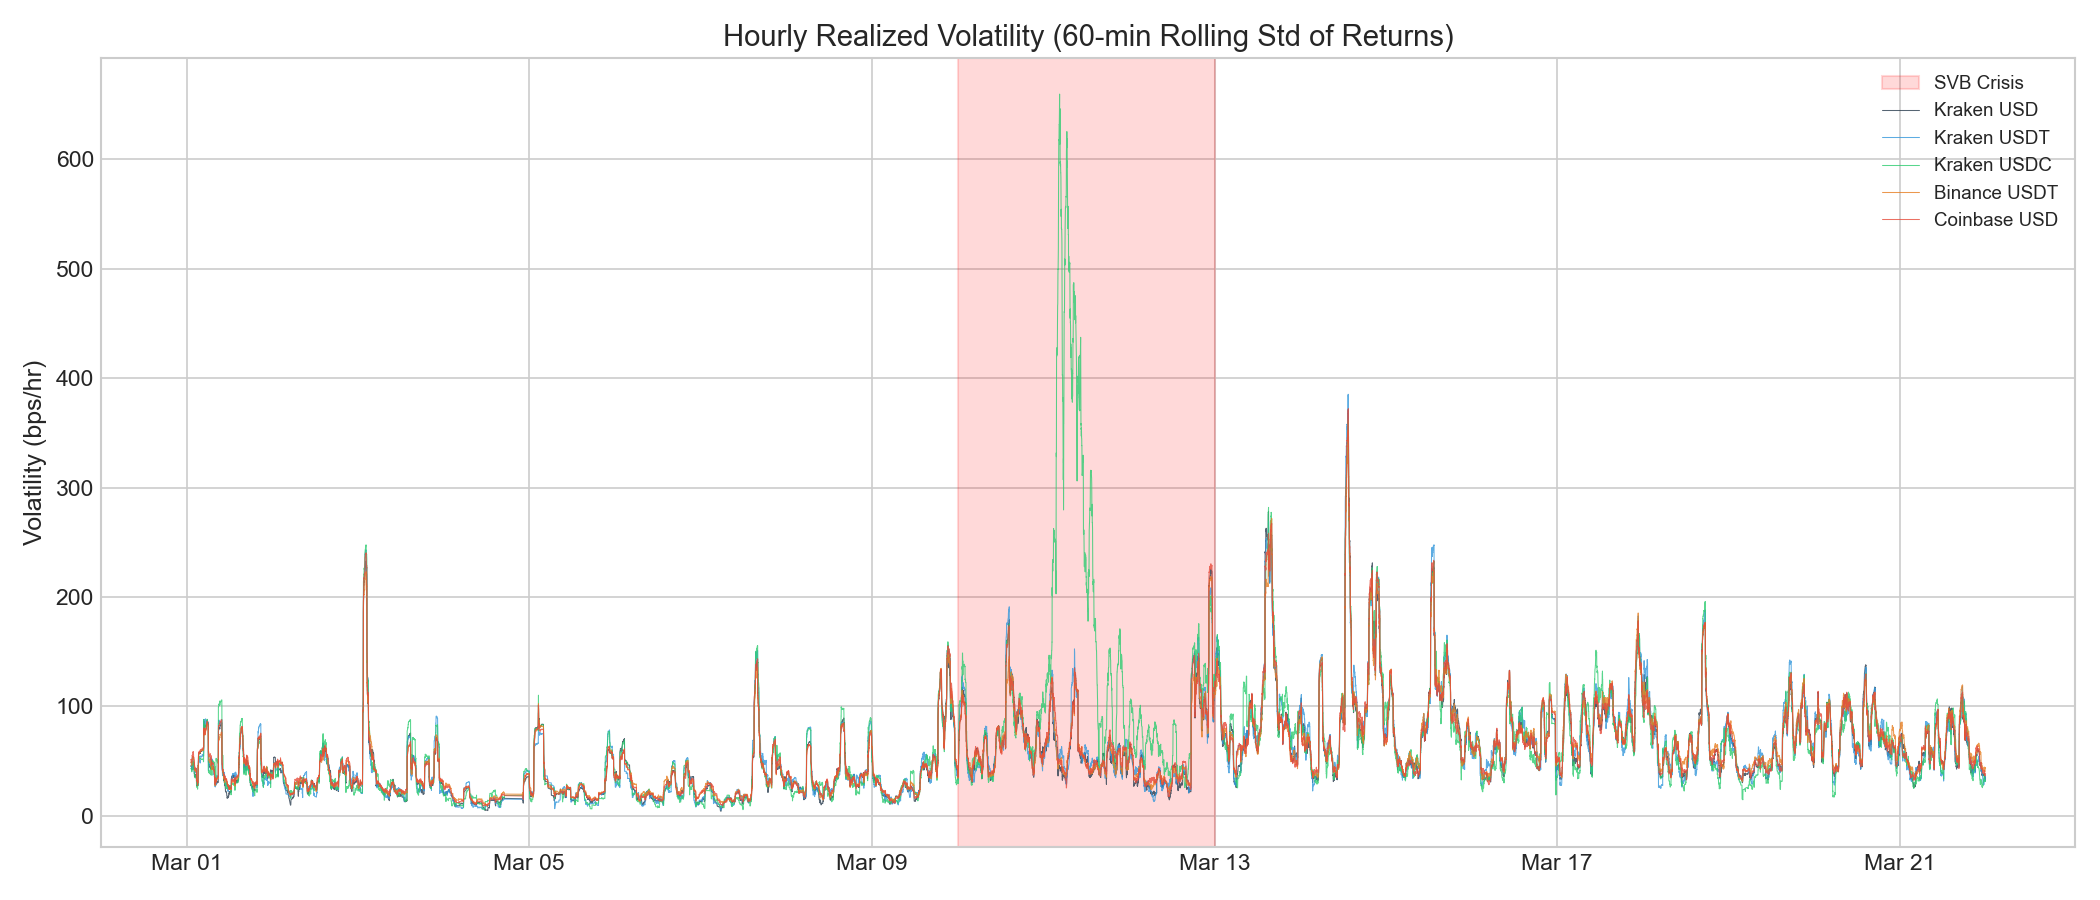
\includegraphics[width=0.82\linewidth]{figures/fig_realized_volatility.png}
    \caption{Hourly realized volatility across BTC pairs. Kraken BTC/USDC spikes to ${\approx}650$ bps/hr during the SVB crisis while USD- and USDT-quoted pairs co-move at ${\approx}150$ bps/hr, demonstrating that the volatility amplification is stablecoin-specific rather than venue-specific.}
    \label{fig:rvol}
\end{figure}

The distributional impact is visible in the adjusted residual $B_t$ (Figure~\ref{fig:bdist}). During the crisis, the USDC $B_t$ distribution shifts rightward (mean $+5.3$ bps) and develops heavy tails extending beyond $\pm100$ bps, compared to a pre-SVB distribution concentrated within $\pm10$ bps; USDT tails widen more modestly. For risk management, this implies that positions denominated in stablecoins carry latent peg-break tail risk that is invisible during calm periods---standard VaR or margin models calibrated on pre-crisis data would severely underestimate the crisis-period exposure. This is precisely the channel that GENIUS Act reserve requirements target: credible, transparent reserves should compress the tail of $B_t$ by removing the confidence-driven component that drives extreme deviations.

\begin{figure}[H]
    \centering
    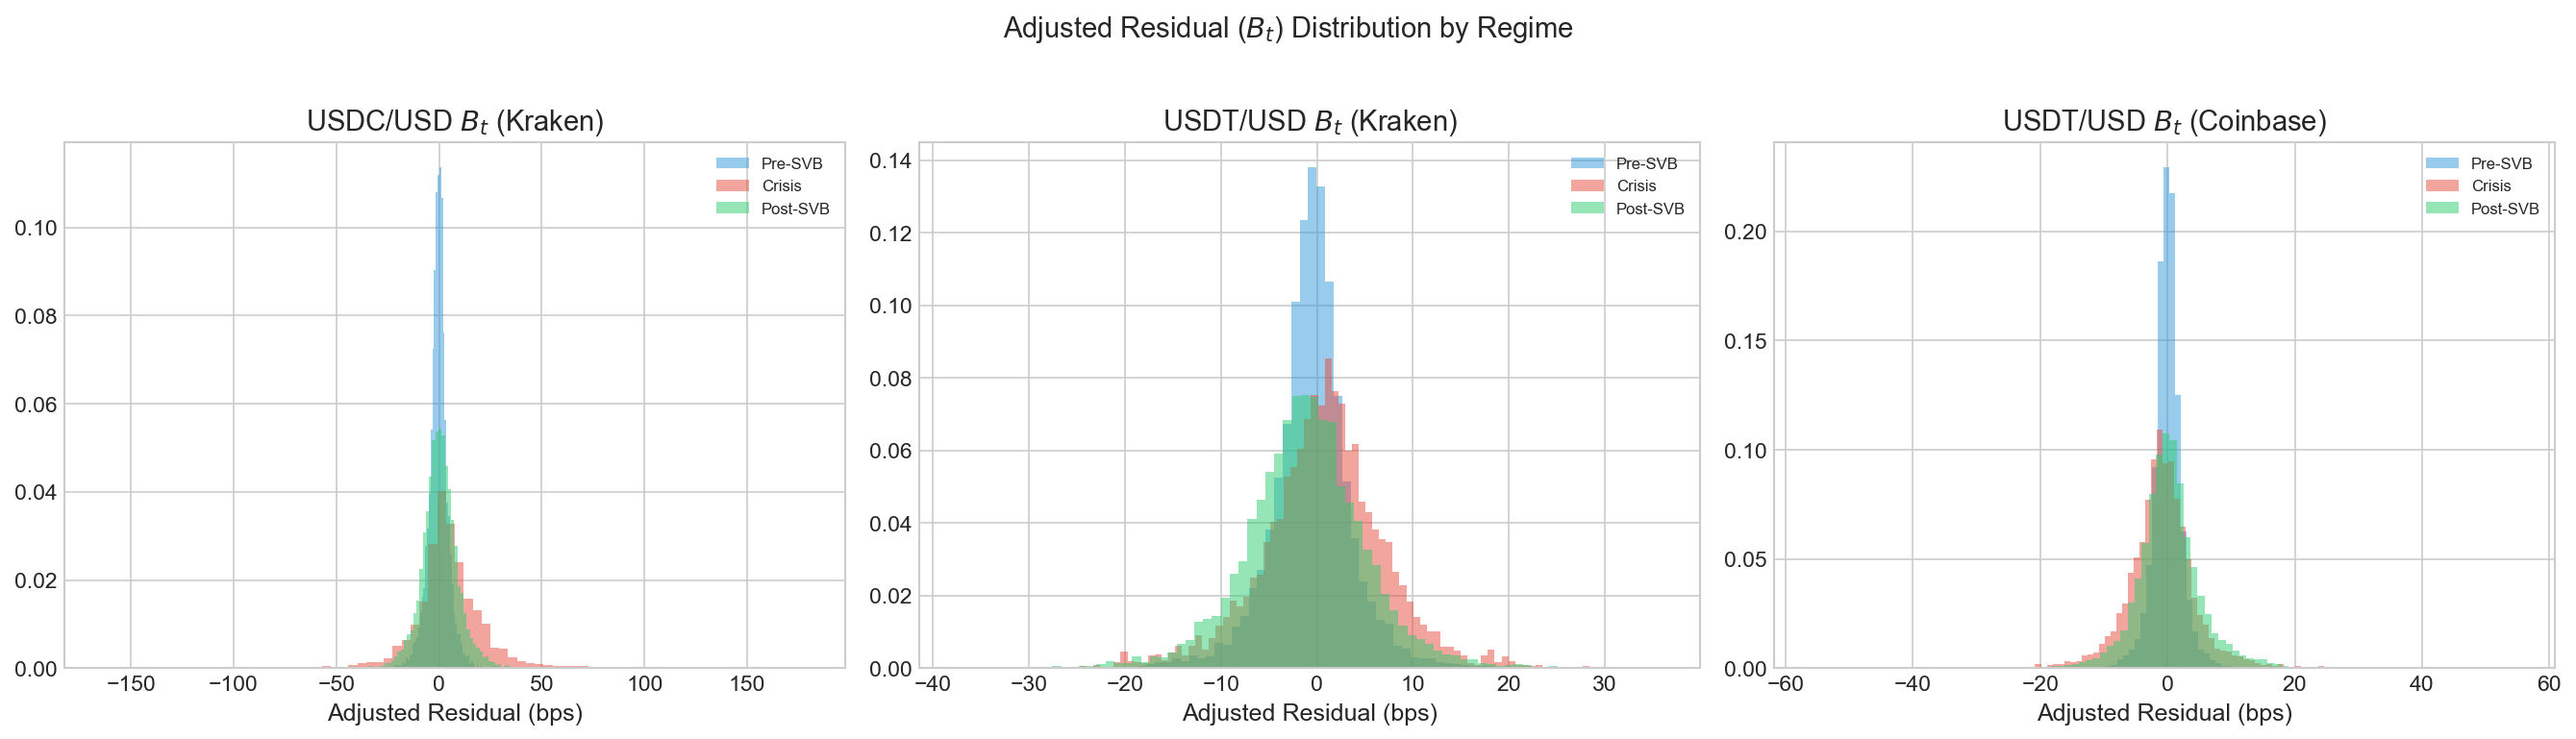
\includegraphics[width=1\linewidth]{figures/fig_basis_distribution.png}
    \caption{Distribution of the adjusted residual $B_t$ by regime. USDC (Kraken) develops heavy tails beyond $\pm100$ bps during the crisis; USDT channels widen modestly. Pre-SVB distributions are tightly concentrated near zero.}
    \label{fig:bdist}
\end{figure}

\subsection{Price discovery}

\begin{table}[H]
\caption{Johansen Cointegration and VECM Adjustment (Primary Kraken Channels, No-FF Sample)}
\label{tab:coint_vecm}
\footnotesize
\centering
\begin{tabular}{lcccccl}
\toprule
Channel & Rank & $k_\Delta$ & Trace$_{r=0}$ & $\alpha_{\text{USD}}$ & $\alpha_{\text{other}}$ & Leader by $|\alpha|$ \\
\midrule
BTC/USD vs BTC/USDC & 0 & 2 & 7.71 & --- & --- & undetermined \\
BTC/USD vs BTC/USDT & 1 & 8 & 27.03 & 0.0079 & 0.0118 & BTC/USD \\
\bottomrule
\multicolumn{7}{l}{\footnotesize 95\% critical value for trace $r=0$: 15.49. Rank stable at $k_\Delta\pm1$ for both channels.}
\end{tabular}
\end{table}


Table~\ref{tab:coint_vecm} shows that Kraken BTC/USD vs.\ BTC/USDT rejects no cointegration (rank $=1$; stable at $k_\Delta\pm1$). We compute Hasbrouck (1995) Information Share (IS) bounds via both Cholesky orderings of the VECM residual covariance $\Sigma_u$: IS$_{\text{USD}}\in[0.69,\,0.77]$, midpoint $\mathbf{0.73}$. BTC/USD therefore accounts for approximately $73\%$ of permanent price discovery. The bounds are tight (width $0.08$), confirming the result is not driven by the Cholesky ordering---BTC/USD is the unambiguous price-discovery leader regardless of which market's innovation is orthogonalized first. This is consistent with the fiat anchor being deeper and more informationally efficient: the residual covariance $\Sigma_u$ shows $\sigma_{\text{USD,USDT}}/\sqrt{\sigma_{\text{USD}}\sigma_{\text{USDT}}}=0.889$, confirming very high co-movement. For BTC/USD vs.\ BTC/USDC, the no-FF specification does not reject rank $=0$: the de-peg episode disrupted any stable long-run relationship, making the 21-day window straddle a structural break.

\begin{sloppypar}
BH/FDR-corrected Granger tests (Table~\ref{tab:granger_fdr}) show directional asymmetry in the USDC channel (BTC/USD $\to$ BTC/USDC significant; reverse not significant after FDR), consistent with fiat-to-stablecoin price adjustment---information flows from the fiat anchor outward, not inward from stablecoin markets. The USDT and cross-exchange channels show bidirectional significance, consistent with active two-way arbitrage in those more liquid and better-functioning channels.
\end{sloppypar}

\input{tables/granger_causality_fdr.tex}

\subsection{Arbitrage after fees}
We evaluate arbitrage using explicit trade construction: 3-leg triangular for intra-exchange stablecoin channels, 2-leg pre-funded buy/sell for cross-exchange. Two cost bounds apply:
\begin{align}
    \text{cost}^{\text{fee}}_t &= n_{\text{legs}}\cdot f, \\
    \text{cost}^{\text{fee+slip}}_t &= n_{\text{legs}}\cdot f + \sum_{\ell=1}^{n_{\text{legs}}}\tfrac{1}{2}\,\text{RangeProxy}_{\ell,t},
\end{align}
with $f=5$ bps per taker leg.

\begin{table}[H]
\caption{Arbitrage Profitability by Channel and Regime (5 bps/leg; 3-leg intra-exchange, 2-leg cross-exchange)}
\label{tab:arb}
\footnotesize
\centering
\begin{tabular}{llcrr}
\toprule
Channel & Regime & Cost Variant & \%Profitable & AvgNet$_{\text{uncond}}$ (bps) \\
\midrule
\multirow{2}{*}{USDC/USD (Kraken)} & \multirow{2}{*}{Crisis} & Fee-only & 29.16 & 4.83 \\
 & & Fee+slip & 6.72 & 0.64 \\
\cmidrule(lr){2-5}
 & \multirow{2}{*}{Post-SVB} & Fee-only & 9.38 & 0.56 \\
 & & Fee+slip & 1.78 & 0.08 \\
\midrule
\multirow{2}{*}{USDT/USD (Kraken)} & \multirow{2}{*}{Crisis} & Fee-only & 3.76 & 0.14 \\
 & & Fee+slip & 0.37 & 0.01 \\
\midrule
\multirow{2}{*}{Cross BTC/USD (CB--KR)} & \multirow{2}{*}{Crisis} & Fee-only & 11.32 & 0.72 \\
 & & Fee+slip & 2.29 & 0.15 \\
\midrule
\multirow{2}{*}{Cross BTC/USDT (BN--KR)} & \multirow{2}{*}{Crisis} & Fee-only & 11.85 & 0.49 \\
 & & Fee+slip & 1.81 & 0.05 \\
\bottomrule
\multicolumn{5}{l}{\footnotesize Pre-SVB rows omitted (near-zero profitability). Full regime matrix available in repo CSV outputs.}
\end{tabular}
\end{table}


\begin{figure}[H]
    \centering
    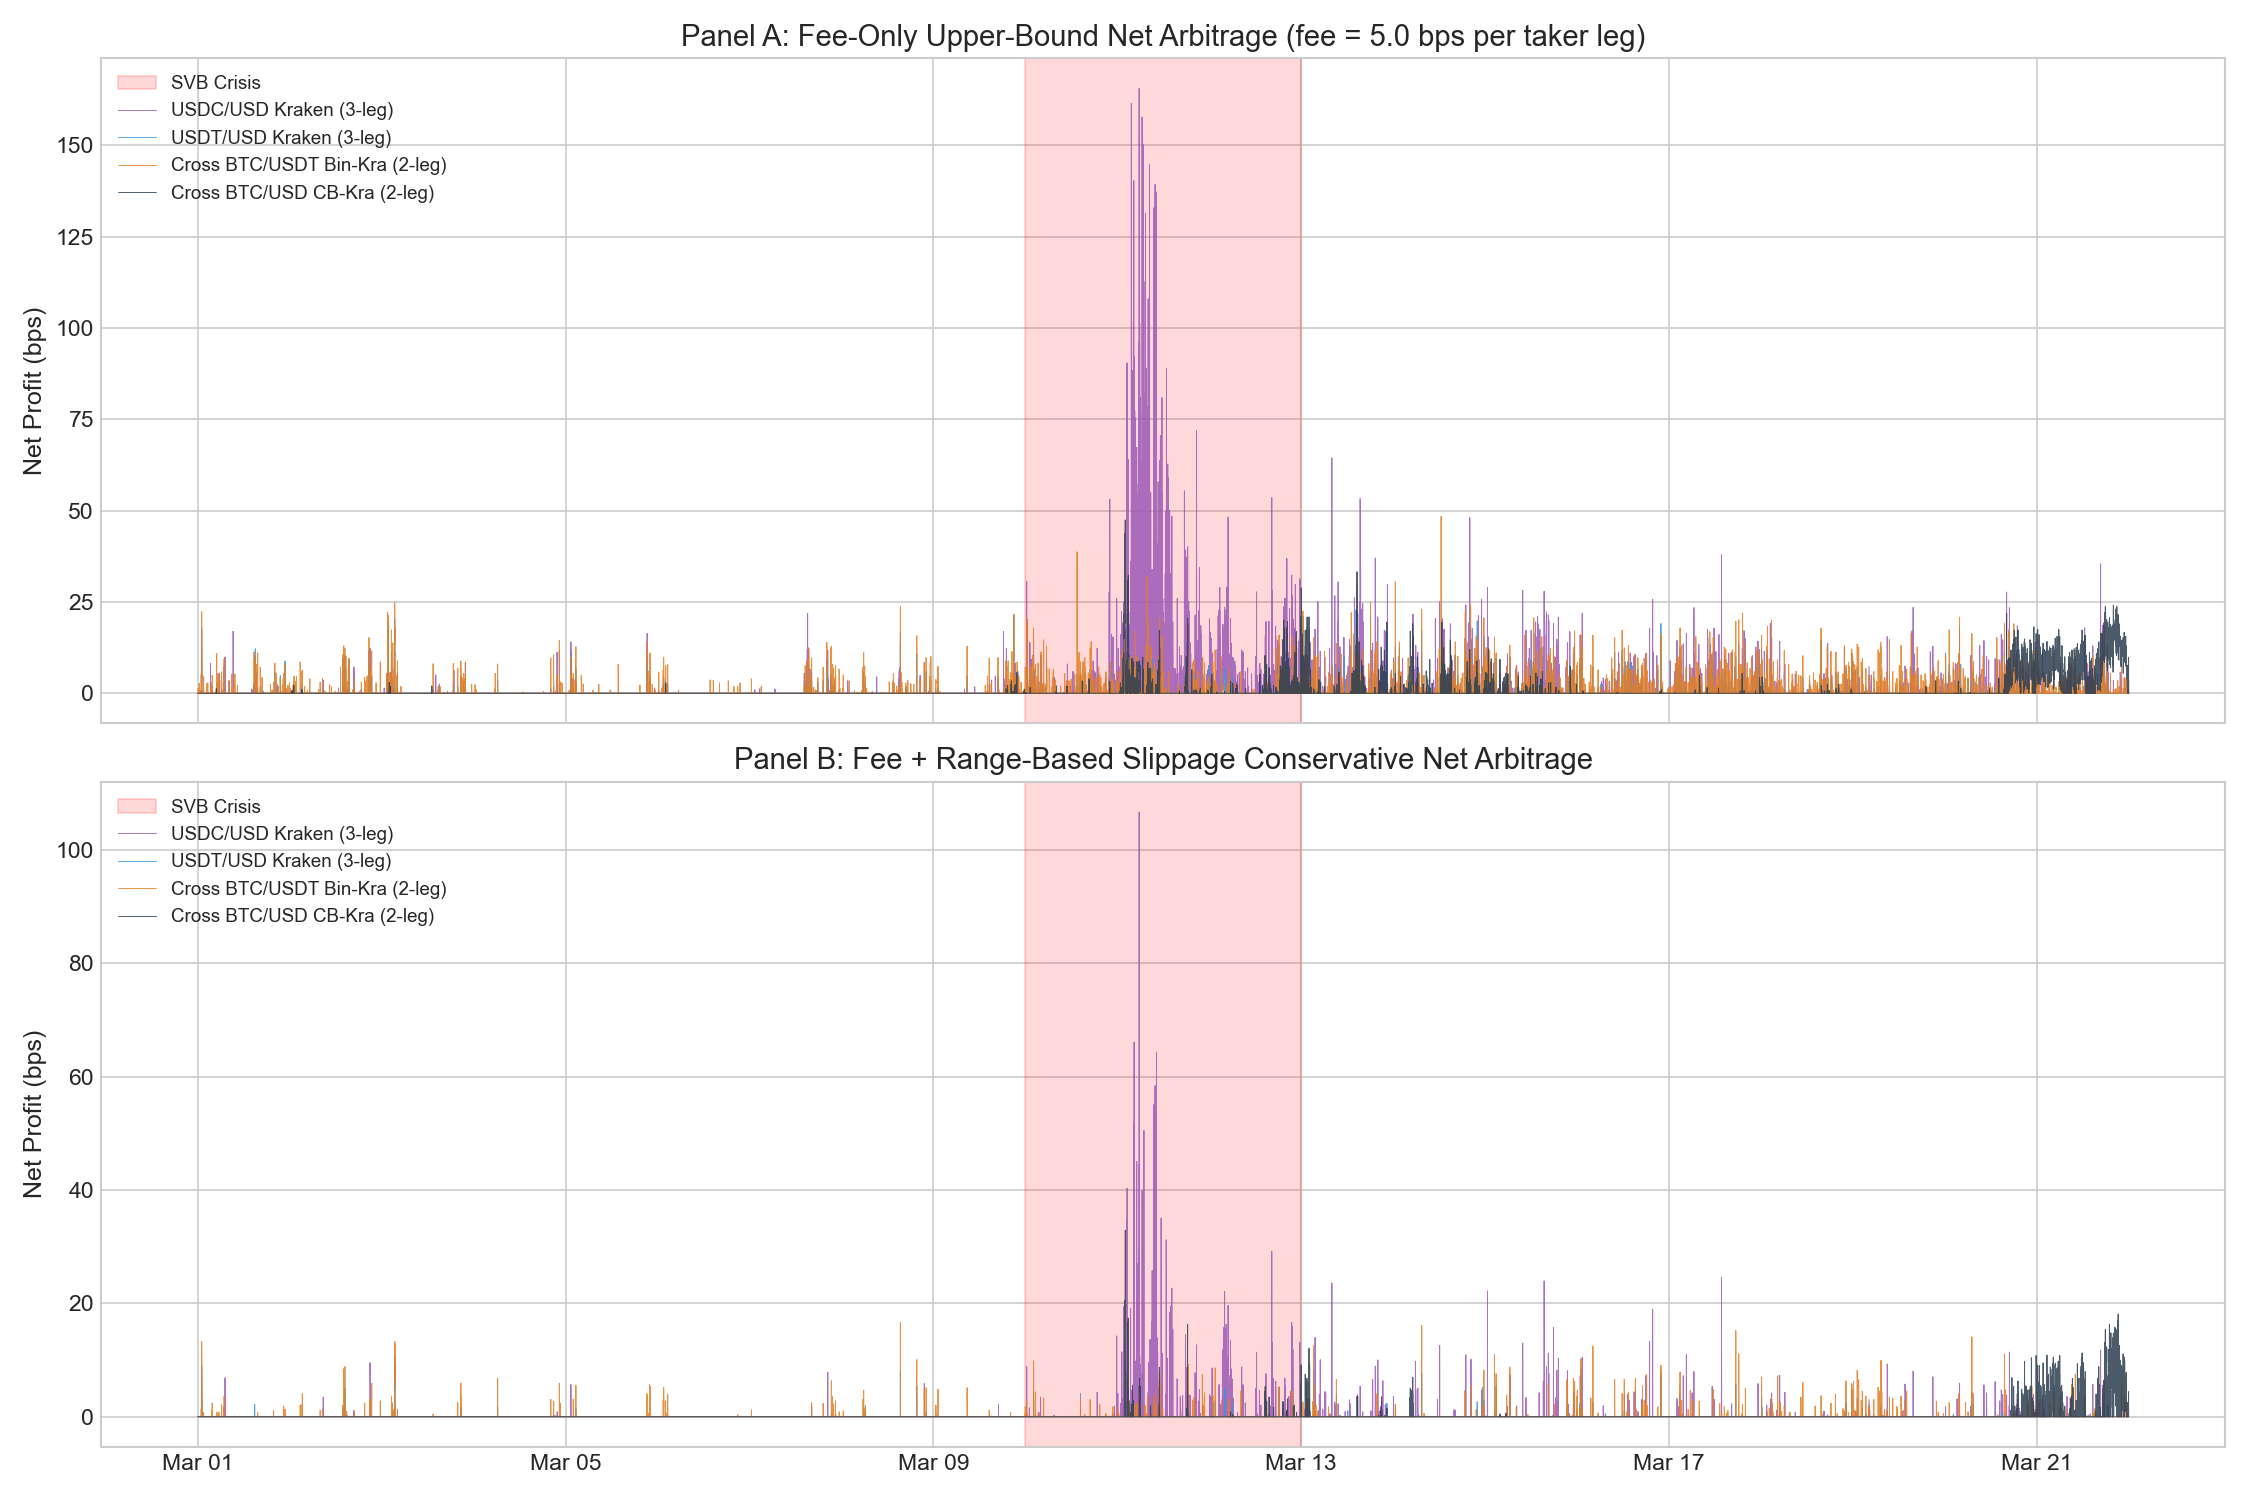
\includegraphics[width=0.82\linewidth]{figures/fig_arbitrage_after_fees.png}
    \caption{Net arbitrage opportunity under fee-only (Panel A) and fee + slippage (Panel B) bounds.}
    \label{fig:arb}
\end{figure}

The fee-only specification is an optimistic upper bound. Adding range-based slippage materially reduces both frequency and net capture: USDC crisis profitability falls from 29.16\% to 6.72\% (unconditional net 4.83 to 0.64 bps); Coinbase--Kraken BTC/USD crisis falls from 11.32\% to 2.29\%. Cross-exchange results assume pre-funded inventory and abstract from transfer delays and exchange-specific fee tiers. The narrow net opportunities even at peak stress confirm that the market, while fragmented, was not generating free money---professional arbitrageurs faced genuine frictions and capital constraints.

\section{Regulatory Interpretation}

The SVB episode suggests that a large share of the cross-currency fragmentation we document was linked to banking-layer reserve-access risk, rather than on-chain market mechanics alone. Circle held \$3.3B of its ${\approx}$\$40B USDC reserves (${\approx}8\%$) at SVB. When SVB failed on Friday evening March 10, those reserves became temporarily inaccessible and USDC holders had no guaranteed redemption timeline. This confidence shock coincided with the \$0.87 de-peg and the $+320$ bps dispersion blowout we document. The peg did not fully recover until March 17, after the Federal Reserve announced emergency deposit guarantees and Circle secured alternative banking arrangements.

The GENIUS Act (signed July 2025) addresses this failure chain through four reinforcing provisions, each mapping to a specific channel in our results. First, \emph{reserve composition requirements} mandate one-to-one backing exclusively in Treasury bills, FDIC-insured deposits, central bank reserves, and Treasury-backed repos. Table~\ref{tab:genius_cf} reports an \emph{illustrative scenario analysis} (not a structural causal estimate): had Circle been required to hold reserves in T-bills and central bank facilities rather than uninsured bank deposits, the \$3.3B at SVB ($8.25\%$ of total reserves) would likely have faced much lower lock-up risk, and crisis $D_t$ would plausibly have been far closer to its pre-crisis level than the observed $+319.97$ bps. Second, \emph{on-demand par redemption within two business days} should damp panic amplification loops: during the SVB weekend, holders could not redeem, turning a reserve-access problem into the market-wide pricing dislocation we document. Third, \emph{bankruptcy super-priority} should reduce extreme $B_t$ tail risk such as the expansion beyond $\pm100$ bps observed during the crisis (Figure~\ref{fig:bdist}).

\begin{table}[H]
\caption{GENIUS Act quantitative counterfactual. Under reserve composition rules (T-bills, central bank reserves, Treasury-backed repos), Circle's \$3.3B held at SVB would have been in instruments immune to bank failure, eliminating the reserve lock-up that caused the USDC de-peg. Counterfactual $D_t$ is bounded by the pre-crisis level.}
\label{tab:genius_cf}
\footnotesize
\resizebox{\textwidth}{!}{%
\begin{tabular}{p{3.5cm}p{3.2cm}p{3.4cm}p{4.6cm}}
\toprule
Metric & Observed (No GENIUS Act) & Counterfactual (GENIUS Act) & Relevant Provision \\
\midrule
Circle reserves at SVB & \$3.3B locked (8.3\%) & \$0 locked (0\%) & Reserve composition: T-bills/CB reserves only \\
$D_t$ crisis mean (USDC) & $+319.97$ bps & $\approx +0.12$ bps (pre-crisis level) & Reserve composition $\Rightarrow$ no de-peg \\
$D_t$ crisis std (USDC) & $322.87$ bps & $\approx 4.95$ bps & Transparency (no information-driven panic) \\
$B_t$ P99 crisis (USDC) & $+81.4$ bps & $\approx +13.6$ bps (pre-crisis P99) & Bankruptcy super-priority + redemption guarantee \\
\bottomrule
\end{tabular}%
}
\end{table}


Fourth, \emph{transparency} closes the information channel. The GENIUS Act mandates monthly public disclosure of reserve composition with CEO/CFO certification. During the SVB crisis, traders did not know USDC's bank exposure until Circle's Friday-night announcement; this asymmetry is consistent with the sharp divergence between USDC ($D_t=+320$ bps) and USDT (crisis premium $+58.1$ bps on Kraken, $+59.7$ bps on Coinbase)---the same flight-to-quality rotation reflected in our Roll spread, Amihud ILLIQ, and volume evidence.

The persistence of cross-exchange fiat deviations post-crisis (Coinbase--Kraken BTC/USD $+2.18$ bps) shows that reserve-layer reforms alone do not eliminate spatial fragmentation. The GENIUS Act's interoperability mandate (federal regulators to prescribe standards via NIST) and Visa's USDC settlement initiative---which provides 24/7 on-chain settlement including weekends, directly closing the Friday-night liquidity gap that amplified the SVB crisis---should compress the execution frictions that kept post-fee arbitrage windows narrow even at peak stress. The open question is whether these provisions are sufficient or whether consolidated cross-venue price feeds and unified clearing are also needed.

\section{Conclusion}

This paper decomposes the cross-currency pricing fragmentation triggered by the SVB crisis into a large stablecoin-driven component ($D_t=+320$ bps for USDC) and a small residual ($B_t=+5.3$ bps) that mean-reverts within one minute---demonstrating that arbitrageurs rapidly corrected mispricing once the stablecoin peg shift is stripped out, but could not prevent the peg-driven dislocation itself. The simultaneous USDT safe-haven premium, volume migration toward fiat and USDT pairs, USDC-specific volatility amplification ($4\times$ peak realized volatility), and heavy-tailed $B_t$ distributions confirm a system-wide flight-to-quality response affecting prices, liquidity, volatility, and risk simultaneously. Hasbrouck (1995) Information Shares assign $73\%$ of permanent price discovery to BTC/USD (bounds $[0.69,\,0.77]$), with information flowing unidirectionally from fiat to stablecoin markets.

These findings support a clear policy implication: the GENIUS Act's reserve composition, redemption guarantee, transparency, and bankruptcy super-priority provisions are directionally aligned with the failure chain highlighted by the SVB episode---reserve inaccessibility, information asymmetry, confidence stress, and peg instability. A natural next step is a post-GENIUS replication study during the next stress event, testing whether the Act's provisions compress $D_t$ and $B_t$ tails, attenuate flight-to-quality rotation, and narrow cross-venue arbitrage windows relative to the SVB baseline. The open question is whether reserve-layer reforms alone are sufficient, or whether additional market-structure measures---cross-chain interoperability mandates, consolidated cross-venue price feeds, or unified clearing for stablecoin-settled trades---are needed to eliminate the residual spatial fragmentation that persists even in fiat channels.

\end{document}
